\documentclass[a4paper,11pt,titlepage]{article}
\usepackage[T1]{fontenc}
\usepackage[utf8]{inputenc}
\usepackage[frenchb]{babel}
\usepackage{lmodern}
\usepackage[final,expansion=true,protrusion=true]{microtype}
\usepackage[top=25mm,bottom=25mm,left=20mm,right=20mm]{geometry}
\usepackage[hidelinks,unicode]{hyperref}
\usepackage{fancyhdr}
\usepackage{graphicx}

\author{Laurent Girod \href{mailto:laurent.girod@heig-vd.ch}{\texttt{<laurent.girod@heig-vd.ch>}}\\
	Karel Ngueukam Djeuda Wilfried \href{wilfried.ngueukamdjeuda@heig-vd.ch}{\texttt{<wilfried.ngueukamdjeuda@heig-vd.ch>}}\\
	Rick Wertenbroek \href{mailto:rick.wertenbroek@heig-vd.ch}{\texttt{<rick.wertenbroek@heig-vd.ch>}}\\
	Cyrill Zundler \href{mailto:cyrill.zundler@heig-vd.ch}{\texttt{<cyrill.zundler@heig-vd.ch>}}
}
\date{\today}
\title{BDR\\Laboratoire no. 5}

\lhead{Laurent Girod\quad{}Karel Ngueukam Djeuda Wilfried\\Rick Wertenbroek\quad{}Cyrill Zundler}
\chead{RES---lab. 05}
\rhead{\today}
\lfoot{}
\cfoot{\thepage}
\rfoot{}

\pagestyle{fancy}

\setcounter{secnumdepth}{2}
\setcounter{tocdepth}{4}

\begin{document}
\maketitle
\tableofcontents
\newpage

\section[Introduction]{Introduction\protect\footnote{Fortement inspiré de \texttt{README.md} fourni dans le cadre de ce laboratoire.}}
Le but principal de ce laboratoire est d'apprendre à mettre en place une architecture web, et de se familiariser avec
des différents composants, tels que les serveurs HTTP, les \emph{load balancers} ou les \emph{reverse proxies}.

Il est également nécessaire de mettre en place un système de découverte automatique de services permettant de ``voire''
si un serveur HTTP est apparu ou a disparu de l'infrastructure et a réagir a ces changement en modifiant
automatiquement la configuration du \emph{load balancer}.

Le tout est fait dans un environnement virtualisé en utilisant \emph{Vagrant} et \emph{Docker}. 

\section{Architecture du système}
Après nous être concertés pour déterminer le genre de services offerts par l'architecture web, nous nous sommes entendus
pour créer un distributeur de citations générées par le programme UNIX \emph{fortune}.
\begin{figure}[h!]
	\centering
	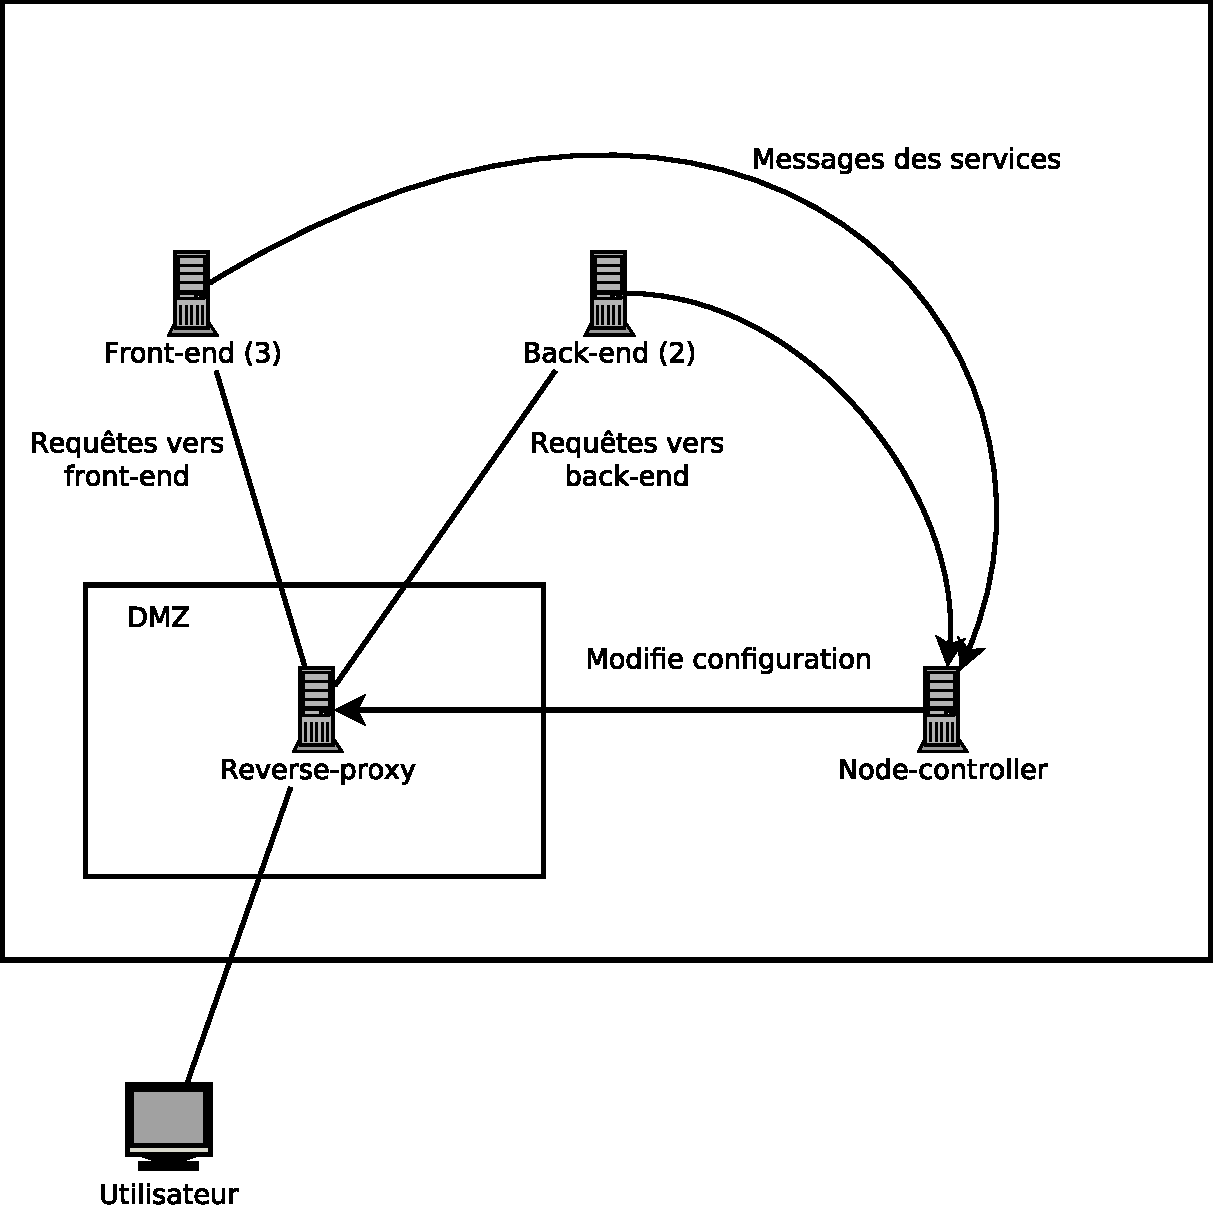
\includegraphics[scale=0.5]{schema.pdf}
	\caption{Architecture du système}
\end{figure}

\subsection{Détails des container}
\subsubsection{\emph{Back-end}}
Le \emph{back-end} est un serveur HTTP répondant à chaque requête par un JSON contenant une citation et
l'adresse IP du back-end selon le motif suivant:
\begin{center}
\texttt{\{"quote":"<citation>","ip":"<IP du backend>"\}}
\end{center}
L'utilité de fournir l'adresse IP est de donner une preuve au testeur que le \emph{load-balancer} (décrit ci-après)
fonctionne correctement.

Afin d'avoir un système le plus léger possible, et qui soit aisé à implémenter, le \emph{back-end} à été réalisé en
javascript avec \emph{Node.js}.

\subsubsection{\emph{Front-end}}
Le \emph{front-end} est un serveur HTTP répondant à chaque requête par un page HTML contenant un javascript permettant
de faire une requête pour récupérer une citation. Cette requête sera redirigée vers le back-end par le
\emph{reverse-proxy}. Afin de fournir une preuve au testeur que le \emph{load-balancer} fonctionne correctement, la page
HTML générée contient l'adresse IP du \emph{front-end}.

Pour les même raisons que pour le \emph{back-end}, le \emph{front-end} à été réalisé en javascript avec \emph{Node.js}.
Notons aussi, que ce serveur est une implémentation minimale conçue dans le cadre de ce laboratoire, et devrait être
grandement améliorée pour toutes utilisation réelle.

\subsubsection{\emph{Node controller}}

\subsubsection{\emph{Reverse proxy et load balancer}}
Nous avons choisi d'implémenter ce point grâce au service httpd (apache2).
Le reverse proxy est le seul point d'entrée extérieur à notre architecture. En effet il sert à masquer le fait qu'il y aie plusieurs machines derrière une adresse, il se chargera de transmettre les différentes requêtes au bon endroit et de retourner les réponses. Il fait en même temps la distribution du travail (load balancer) lorsqu'il a plusieurs possibilités vers qui envoyer une requête (parce qu'on a plusieurs machines qui sont capables de faire la même chose, plusieurs frontend et backend) il va choisir de les distribuer équitablement afin de partager le travail. Nous avons choisi ici d'implémenter une méthode "Round-Robin". La communication avec le front-end est en sticky session avec un cookie qui permet de spécifier la route (donc quel frontend) comme ça si un client a commencé à communiquer avec un frontend il va continuer avec ce frontend tant qu'il donne le cookie, si un nouveau client arrive (sans cookie donc) le load balancer va le rediriger au prochain frontend comme indiqué par notre police "Round-Robin".
Le fichier de configuration du reverse proxy - load balancer est généré par le node-controller et est mis à jour à chaque changement dans les services disponibles (nouveau frontend ou backend ou bien si un frontend ou backend n'est plus disponible). Pour rendre effectif la modification nous relançons la machine depuis le node-controller (qui a les privilèges) avec Dockerode, dans le fichier de configuration de httpd il est spécifié de charger notre fichier de configuration spécifique qui est partagé entre le node controller et cette machine-ci.
Note: La route pour la sticky session est l'ID unique du container vers qui la route pointe, ceci nous garantit que si la machine tombe et se relance la route sera conservée, si on utilisais des entier 1,2,3 etc... si la machine 2 tombe et que la machine 3 prends la place du 2 la route 2 renverrait vers une autre machine qu'au par avant. Avec les ID uniques une route ne pointera que vers une seule machine et toujours la même.

\subsection{Protocoles de communications utilisés}

\section{Conclusions}
À la fin de ce laboratoire, nous avons obtenu un système fonctionnel, et se comportant de manière idoine, et fidèle aux
objectifs fixés. Nous avons également appris de manière concrète le fonctionnement d'une architecture web. Nous pouvons
donc en conclure que ce laboratoire est un succès.

\end{document}
